\documentclass[a4paper, 12pt]{article}
\usepackage{style}
\usepackage{hyperref}

%colori per tablle tabu
\definecolor{tableHeader}{RGB}{254, 61, 0}
\definecolor{tableLineOne}{RGB}{245, 245, 245}
\definecolor{tableLineTwo}{RGB}{254, 204, 188}
%define header tabelle tabu
\newcommand{\tableHeaderStyle}{
    \rowfont[c]{\leavevmode\color{white}\bfseries}
    \rowcolor{tableHeader}
}

\title{PianoDiProgetto}
\author{Cyber13}
\date{March 2019}

\begin{document}
	\begin{titlepage}
		\centering Università degli Studi di Padova
		\line(1,0){350}\\
		\vspace{1.2cm}
		\logo
		\vspace{1.0cm}
		\centering{\bfseries\LARGE PIANO DI PROGETTO \\}
		\vspace{0.5cm}
		\centering{\slshape\large Gruppo Cyber13 - Progetto P2PCS\\}
		\vspace{0.5cm}
		\centering{\bfseries Informazioni sul documento \\}
		\line(1,0){240}\\
		% compilare i campi per ogni documento
		\begin{tabular}{r|l}
			{\textbf{Versione}} 			& 1.0.0\\
			{\textbf{Data Redazione}} 	& 11/04/2019\\	% aggiornare la data
			{\textbf{Responsabili}} 	& Matteo Squeri\\ & Andrea Casagrande\\	% aggiornare la data
			{\textbf{Redazione}} 		& Matteo Squeri \\ & Fabio Garavello \\
			{\textbf{Verifica}} 		 & Andrea Casagrande \\ & Daniel Mirel Bira \\ & Ilaria Rizzo\\
			{\textbf{Approvazione}} 	& Andrea Casagrande\\
			{\textbf{Uso}} 				& Esterno\\
			{\textbf{Destinatari}} 	& GaiaGo \\& Cyber13\\ & Prof. Tullio Vardanega\\ & Prof. Riccardo Cardin\\
			{\textbf{Mail di contatto}} 	& swe.cyber13@gmail.com\\
		\end{tabular}\\
	\end{titlepage}

	\newpage
		\subfile{DiarioModifiche.tex}
	\newpage
		\tableofcontents
    \newpage
	    \listoftables
	\newpage
	    \listoffigures
    \newpage
        \section{Introduzione}
        \subsection{Scopo del documento}
Il presente documento ha il compito di descrivere le motivazioni che hanno portato i componenti del team Cyber13 alla scelta dello svolgimento del \citgl{capitolato} C5. La scelta è stata effettuata tenendo conto dei seguenti fattori:
    \begin{itemize}
        \item Le proposte dei vari progetti e quello che richiedono di implementare.
        \item Le tecnologie che i progetti richiedono per il loro sviluppo. Considerando che il gruppo si colloca nel \citgl{secondo lotto} e che la maggioranza degli studenti ha esami arretrati, si è preferito avvantaggiare progetti che proponessero tecnologie almeno in parte conosciute dai componenti.
        \item I progetti ancora disponibili. I progetti non più a disposizione sono stati scartati.
    \end{itemize}
		            
\subsection{Glossario}
Onde evitare ambiguità o incomprensioni di natura lessicale, si allega il \G.
All'interno del documento saranno presenti parole di ambito specifico, uso raro che potrebbero creare incomprensioni. Per una maggiore leggibilità tali parole sono riconoscibili all'interno dei vari documenti in quanto scritte in corsivo e con un 'g' a pedice tra barre orizzontali (per esempio \citgl{Glossario})
    
\subsection{Riferimenti}
    \subsubsection{Riferimenti normativi}
        \begin{itemize}
            \item \NdP
        \end{itemize}
    
    \subsubsection{Riferimenti informativi}
        \begin{itemize}
            \item Capitolato C1:\\ \url{https://www.math.unipd.it/~tullio/IS-1/2018/Progetto/C1.pdf}
            \item Capitolato C2:\\ \url{https://www.math.unipd.it/~tullio/IS-1/2018/Progetto/C2.pdf}
            \item Capitolato C3:\\ \url{https://www.math.unipd.it/~tullio/IS-1/2018/Progetto/C3.pdf}
            \item Capitolato C4:\\ \url{https://www.math.unipd.it/~tullio/IS-1/2018/Progetto/C4.pdf}
            \item Capitolato C5:\\ \url{https://www.math.unipd.it/~tullio/IS-1/2018/Progetto/C5.pdf}
            \item Capitolato C6:\\ \url{https://www.math.unipd.it/~tullio/IS-1/2018/Progetto/C6.pdf}
        \end{itemize}
   
    \newpage
        \section{Modello di sviluppo}
        Come modello di ciclo di vita del software è stato scelto dal gruppo di adottare il \citgl{modello incrementale}. Tale modello prevede che, previa la conoscenza del \citgl{sistema} che si intende implementare, lo sviluppo del progetto venga suddiviso in varie fasi. Il termine di ogni fase definisce una \citgl{milestone}. Ogni fase è a sua volta suddivisa in sotto-attività tali da poter essere affrontate come raffinamenti o estensioni delle attività concluse in precedenza, senza però impattare sul resto del progetto.
\\L'utilizzo del modello incrementale prevede quindi di suddividere il sistema che si intende realizzare in parti più piccole: andranno identificate quelle più critiche ed essenziali, le quali saranno implementate per prime. In questo modo è possibile porre una solida base di partenza: in seguito si procederà incrementalmente fino allo sviluppo del sistema completo. Necessario è porre un limite massimo ben definito al numero di fasi/incrementi, pena il rischio di trasformare il modello incrementale in un loop potenzialmente infinito di iterazioni non incrementali.
\\\\Ad esempio, nella fase di Analisi dei Requisiti del sistema che si intende realizzare è importante distinguere quali di essi siano essenziali, quindi andranno implementati per primi, e quali invece siano solo desiderabili, quindi implementabili in un secondo momento.
\\A questo fine risulta importante la comunicazione con la \citgl{proponente} \citgl{GaiaGo}, il cui massimo coinvolgimento è uno degli obiettivi della pianificazione.

\subsection{Fasi di Progetto}
Per il progetto P2PCS sono state identificate 5 fasi fondamentali. Le attività che compongono ciascuna fase sono descritte e pianificate nella sezione 4 del presente Piano di Progetto:
\begin{itemize}
    \item Analisi: La prima fase è data da tutte quelle attività necessarie ad organizzare il lavoro del team. In particolare consiste nella realizzazione di alcuni documenti ad uso interno ed esterno cui ogni membro dovrà fare riferimento durante le successive fasi di lavoro.
    \item Analisi di dettaglio: Una breve fase intermedia tra la realizzazione dell'Analisi e l'inizio della Progettazione. Necessaria per raffinare e verificare quanto prodotto durante la fase di Analisi in vista della prima consegna del materiale e per presentare il lavoro del team alla \citgl{Proponente} e al \citgl{Committente}.
    \item Progettazione della base tecnologica: Fase di definizione delle tecnologie e delle scelte dei Progettisti e conseguente realizzazione di un prototipo del software sulla base di tali scelte.
    \item Progettazione di dettaglio e codifica: In questa fase viene sviluppato il corpo principale dell'applicativo scopo del progetto. I programmatori scrivono il codice seguendo le direttive dei progettisti, i quali affinano la progettazione del programma a partire dalle basi e le tecnologie descritte nella fase precedente.
    \item Validazione e collaudo: Fase di completamento e raffinamento dell'applicazione, i verificatori si assicurano che il software sviluppato sia conforme ai requisiti individuati dagli analisti e i programmatori incrementano l'applicativo allo scopo di eliminare errori e mancanze riscontrate durante il collaudo. La documentazione, incluso un manuale per l'utilizzo dell'applicazione, vengono rifiniti e completati. Al termine della fase il prodotto finito viene consegnato dal team alla \citgl{Proponente} e al \citgl{Committente} per l'approvazione.
\end{itemize}
Le fasi di Analisi e Progettazione non sono reiterabili: una volta identificati i Requisiti, essi restano fissati. Se così non fosse, non sarebbe possibile pianificare i cicli di incremento. Possibili fattori di rischio che potrebbero causare problemi e discostare il ciclo di sviluppo come pianificato allo scopo di adattarlo al modello incrementale sono riportati e analizzati nella sezione 4 del presente Piano di Progetto.
    \newpage
        \section{Analisi dei rischi}
        Di seguito viene effettuata un'approfondita analisi sui rischi che potrebbero compromettere lo svolgimento del progetto. I rischi vengono divisi per fattore di rischio ed analizzati allo scopo di produrre una breve descrizione e misurare la probabilità di occorrenza e la loro gravità. Per ogni rischio individuato viene proposto un piano di contingenza per scongiurarli oppure cercare di ridurre l'impatto sullo sviluppo se inevitabili.
\subsection{Rischi riguardanti i membri del team}

\begin{table}[H]
\taburowcolors[2] 2{tableLineOne .. tableLineTwo}
\tabulinesep = 10pt
\everyrow{\tabucline[.4mm  white]{}}
\begin{tabu} to \textwidth { X[l,1.5] X[l,4] }
    \tableHeaderStyle
    Nome rischio & Scarsa esperienza \\
    Descrizione & Nessun membro del gruppo ha mai lavorato ad un progetto di tale portata. Molte tecnologie e metodologie utilizzate risultano sconosciute a vari membri. \\
    Individuazione & Ciascun componente comunicherà, dove rilevante, le proprie mancanze relativamente ai compiti assegnati. \\
    Occorrenza & Alta \\
    Gravità & Alta \\
    Piano di contingenza & I compiti saranno assegnati ai membri che hanno esperienza in merito. Se ciò non fosse possibile, i membri del gruppo offriranno supporto al componente in difficoltà nel caso specifico. \\
\end{tabu}
\caption{Rischio: Scarsa esperienza}
\end{table}

\begin{table}[H]
\taburowcolors[2] 2{tableLineOne .. tableLineTwo}
\tabulinesep = 10pt
\everyrow{\tabucline[.4mm  white]{}}
\begin{tabu} to \textwidth { X[l,1.5] X[l,4] }
    \tableHeaderStyle
    Nome rischio & Contrasti tra i membri del gruppo \\
    Descrizione & Essendo il gruppo stato formato in modo causale molti membri non hanno mai collaborato ad un progetto. Questa mancanza di conoscenza tra i membri potrebbe portare a tensioni e conflitti sulle modalità di avanzamento dello sviluppo. \\
    Individuazione & Sarà compito del responsabile controllare la collaborazione tra i componenti del gruppo. In caso di problemi con altri componenti, questi saranno comunicati al responsabile se non viene trovata una soluzione indipendentemente. \\
    Occorrenza & Bassa \\
    Gravità & Media \\
    Piano di contingenza & Si cercherà di mantenere separati membri che presentano frequenti contrasti, assegnandoli ad attività diverse.\\
\end{tabu}
\caption{Rischio: Contrasti tra i membri del gruppo}
\end{table}

\begin{table}[H]
\taburowcolors[2] 2{tableLineOne .. tableLineTwo}
\tabulinesep = 10pt
\everyrow{\tabucline[.4mm  white]{}}
\begin{tabu} to \textwidth { X[l,1.5] X[l,4] }
    \tableHeaderStyle
    Nome rischio & Mancanza di disponibilità dei membri \\
    Descrizione & Alcuni membri del gruppo sono studenti lavoratori, quindi il tempo che possono dedicare al progetto è limitato. Inoltre, vista la durata del progetto, questo potrebbe sovrapporsi ad altre attività universitarie a carico dei componenti. \\
    Individuazione & Ogni membro comunicherà con sufficiente anticipo al responsabile i giorni in cui non potrà portare avanti i compiti assegnati.  \\
    Occorrenza & Alta \\
    Gravità & Media \\
    Piano di contingenza & Il carico di lavoro verrà redistribuito tra i membri con maggiore disponibilità di tempo. L'obiettivo rimarrà quello di non far slittare la data di completamento dell'attività. \\
\end{tabu}
\caption {Rischio: Mancanza di disponibilità dei membri}
\end{table}

\begin{table}[H]
\taburowcolors[2] 2{tableLineOne .. tableLineTwo}
\tabulinesep = 10pt
\everyrow{\tabucline[.4mm  white]{}}
\begin{tabu} to \textwidth { X[l,1.5] X[l,4] }
    \tableHeaderStyle
    Nome rischio & Perdita di motivazione \\
    Descrizione &  Data l'estesa durata del progetto è possibile che alcuni membri del gruppo possano perdere motivazione nello svolgimento dei loro compiti, portando a ritardi nello sviluppo.\\
    Individuazione & Sarà compito del responsabile supervisionare il lavoro svolto dai membri del gruppo, notando eventuali ritardi non giustificati nell'avanzamento. \\
    Occorrenza & Bassa\\
    Gravità & Bassa \\
    Piano di contingenza & Il responsabile si occuperà di parlare personalmente con i membri del gruppo in cui ha notato mancanza di impegno nello sviluppo, ricordando loro gli impegni presi.\\
\end{tabu}
\caption{Rischio: Perdita di motivazione}
\end{table}

\subsection{Rischi riguardanti l'organizzazione}

\begin{table}[H]
\taburowcolors[2] 2{tableLineOne .. tableLineTwo}
\tabulinesep = 10pt
\everyrow{\tabucline[.4mm  white]{}}
\begin{tabu} to \textwidth { X[l,1.5] X[l,4] }
    \tableHeaderStyle
    Nome rischio & Sottostima dei costi e dei tempi \\
    Descrizione & Data l'inesperienza in campo organizzativo lungo una durata temporale così ampia da parte del responsabile, è possibile fare delle assunzioni sbagliate nella pianificazione. Può accadere che i tempi dedicati a ciascuna attività si rivelino sottostimati creando quindi problemi nella gestione dell'intero progetto. \\
    Individuazione & Il responsabile verificherà periodicamente lo stato dell'attività e i membri si aggiorneranno costantemente sullo stato dell'avanzamento.\\
    Occorrenza & Media \\
    Gravità & Alta \\
    Piano di contingenza & In caso di ritardi importanti il responsabile modificherà la pianificazione, ridistribuendo il carico lavorativo tra i membri in anticipo sulla data di scadenza per le attività a loro assegnate. \\
\end{tabu}
\caption{Rischio: Valutazione dei costi e dei tempi}
\end{table}

\begin{table}[H]
\taburowcolors[2] 2{tableLineOne .. tableLineTwo}
\tabulinesep = 10pt
\everyrow{\tabucline[.4mm  white]{}}
\begin{tabu} to \textwidth { X[l,1.5] X[l,4] }
    \tableHeaderStyle
    Nome rischio & Comunicazione con la proponente \\
    Descrizione & Durante lo sviluppo il gruppo si impegna a contattare la proponente al fine di stabilire con più chiarezza le funzionalità richieste dal prodotto. Tuttavia potrebbero verificarsi momenti di stallo e incertezza dovuti alla mancanza di disponibilità della proponente, per suoi impegni, di comunicare col team.  \\
    Individuazione & Il responsabile cercherà di stabilire le date per mettersi in contatto con la proponente a seconda della disponibilità di quest'ultima. Al responsabile spetta anche il comunicare al gruppo quando la proponente non risulta più disponibile per una data prefissata. \\
    Occorrenza & Bassa \\
    Gravità & Media \\
    Piano di contingenza & In caso di spostamento di un incontro con la proponente riguardo un argomento di fondamentale importanza per l'avanzamento di alcune attività il responsabile negozierà una nuova data e redistribuirà i membri su attività per le quali non siano attese ulteriori informazioni. \\
\end{tabu}
\caption{Rischio: Comunicazione con la proponente}
\end{table}

\subsection{Rischi riguardanti i requisiti}

\begin{table}[H]
\taburowcolors[2] 2{tableLineOne .. tableLineTwo}
\tabulinesep = 10pt
\everyrow{\tabucline[.4mm  white]{}}
\begin{tabu} to \textwidth { X[l,1.5] X[l,4] }
    \tableHeaderStyle
    Nome rischio & Comprensione dei requisiti \\
    Descrizione & È possibile che durante l'analisi del capitolato alcuni requisiti individuati siano errati o che altri vengano invece tralasciati. \\
    Individuazione & Uno degli obiettivi del team è di comunicare il più possibile con la proponente al fine di evitare problematiche riguardanti la corretta comprensione dei requisiti. Questo permette una più immediata rilevazione di errori nei requisiti o mancanza degli stessi. \\
    Occorrenza & Media \\
    Gravità & Media \\
    Piano di contingenza & Verranno discussi in dettaglio i requisiti che presentano più problemi di comprensione con la proponente.\\
\end{tabu}
\caption{Rischio: Comprensione dei requisiti}
\end{table}

\begin{table}[H]
\taburowcolors[2] 2{tableLineOne .. tableLineTwo}
\tabulinesep = 10pt
\everyrow{\tabucline[.4mm  white]{}}
\begin{tabu} to \textwidth { X[l,1.5] X[l,4] }
    \tableHeaderStyle
    Nome rischio & Cambiamenti nei requisiti \\
    Descrizione & È possibile che la proponente voglia apportare delle modifiche ai requisiti già individuati nel corso dello sviluppo. Questo potrebbe portare ad una modifica importante del documento Analisi dei Requisiti e creare problemi alla pianificazione delle attività. \\
    Individuazione & Si ritiene necessario lavorare da subito a stretto contatto con la proponente al fine di stabilire con certezza i requisiti, ed individuare il prima possibile eventuali modifiche.    \\
    Occorrenza & Bassa \\
    Gravità & Alta \\
    Piano di contingenza & In caso venga richiesto un cambiamento sostanzioso dei requisiti rispetto a quelli già individuati, questo verrà discusso da tutto il gruppo con la proponente al fine di minimizzare l'impatto negativo che ciò avrebbe sull'avanzamento. \\
\end{tabu}
\caption{Rischio: Cambiamenti nei requisiti}
\end{table}

\subsection{Rischi riguardanti le tecnologie}

\begin{table}[H]
\taburowcolors[2] 2{tableLineOne .. tableLineTwo}
\tabulinesep = 10pt
\everyrow{\tabucline[.4mm  white]{}}
\begin{tabu} to \textwidth { X[l,1.5] X[l,4] }
    \tableHeaderStyle
    Nome rischio & Tecnologie richieste per lo sviluppo \\
    Descrizione & Le tecnologie necessarie per lo sviluppo di alcune funzionalità sono relativamente recenti e in alcuni casi molto specifiche. Il tempo di apprendimento di queste tecnologie potrebbe causare ritardi nell'avanzamento. \\
    Individuazione & Il responsabile dovrà verificare la preparazione dei vari membri in relazione alle attività a loro assegnate. Se dovesse esserci una grave mancanza di competenza da parte di un membro questo dovrà farlo sapere al responsabile. \\
    Occorrenza & Alta \\
    Gravità & Media \\
    Piano di contingenza & In caso di gravi mancanze il responsabile potrebbe considerare di riservare più tempo allo studio di una specifica tecnologia, possibilmente includendo altri membri più esperti nell'apprendimento.\\
\end{tabu}
\caption{Rischio: Tecnologie richieste per lo sviluppo}
\end{table}

\subsection{Rischi riguardanti gli strumenti}

\begin{table}[H]
\taburowcolors[2] 2{tableLineOne .. tableLineTwo}
\tabulinesep = 10pt
\everyrow{\tabucline[.4mm  white]{}}
\begin{tabu} to \textwidth { X[l,1.5] X[l,4] }
    \tableHeaderStyle
    Nome rischio & Problematiche software \\
    Descrizione & Il gruppo fa riferimento a software di terze parti o servizi online, ad esempio \citgl{Github}, e un malfunzionamento di questi potrebbe portare a errori o alla perdita di materiale.  \\
    Individuazione & Difficile prevedere e rilevare questo genere di problematiche dato che spesso non dipendono in alcun modo dai membri del gruppo. \\
    Occorrenza & Bassa \\
    Gravità & Media \\
    Piano di contingenza & Gli strumenti scelti dal gruppo sono considerati molto affidabili, tuttavia data l'importanza dei dati prodotti dal team verranno effettuati backup frequenti per minimizzare la portata di eventuali errori.\\
\end{tabu}
\caption{Rischio: Problematiche software}
\end{table}

\begin{table}[H]
\taburowcolors[2] 2{tableLineOne .. tableLineTwo}
\tabulinesep = 10pt
\everyrow{\tabucline[.4mm  white]{}}
\begin{tabu} to \textwidth { X[l,1.5] X[l,4] }
    \tableHeaderStyle
    Nome rischio & Problematiche hardware \\
    Descrizione & Ogni membro utilizza il proprio pc personale per svolgere gli incarichi assegnati. Eventuali guasti potrebbero portare a ritardi nell'avanzamento o perdita di materiale. La portata di questa problematica è abbastanza ridotta data la disponibilità di computer secondari da parte dei membri del gruppo e il forte utilizzo di servizi di memorizzazione dati online. \\
    Individuazione & Il membro del gruppo che ha riscontrato un guasto nei propri strumenti dovrà avvisare il prima possibile il responsabile. \\
    Occorrenza & Bassa \\
    Gravità & Bassa \\
    Piano di contingenza & Ogni membro del gruppo dovrà effettuare frequenti backup di tutti i files relativi al progetto. In caso di temporanea impossibilità a procedere con i propri compiti dovuta a un guasto del pc il gruppo si impegnerà a fornire un dispositivo sostitutivo dove possibile.\\
\end{tabu}
\caption{Rischio: Problematiche hardware}
\end{table}

    \newpage
        \section{Pianificazione}
        La pianificazione è stata stilata in base alle scadenze preventivate al punto 1.4 del documento. Si è deciso di dividere il processo di sviluppo in cinque fasi:
\begin{itemize}
    \item \textbf{Analisi};
    \item \textbf{Analisi di dettaglio};
    \item \textbf{Progettazione della base tecnologica};
    \item \textbf{Progettazione di dettaglio e codifica};
    \item \textbf{Validazione e collaudo}.
\end{itemize}
Ogni fase prevede periodi di incremento e successiva validazione delle attività in essa previste. Questi verranno riportati in \citgl{diagrammi di Gantt}, ciascuno dedicato ad una fase specifica. Per ogni fase e rispettive attività verranno indicati i ruoli che contribuiranno all'avanzamento. La scadenza di ogni fase è segnata come \citgl{milestone}.
\subsection{Analisi}
La fase di Analisi ha inizio in data 04-03-2019 e termina il 01-04-2019. I ruoli attivi in questa fase sono:
\begin{itemize}
    \item \textbf{Responsabile di progetto};
    \item \textbf{Amministratore};
    \item \textbf{Verificatore};
    \item\textbf{Analista}.
\end{itemize}
Le attività svolte in questa fase sono:
\begin{itemize}
    \item \textbf{Norme di Progetto}: Consiste nella stesura di un documento da parte degli Amministratori. Questa attività ha la priorità e risulta bloccante all'inizio delle altre attività previste in questa fase, ad eccezione dell'incremento del Glossario. Ciò è dovuto alla natura del documento, che consiste nella stesura di una serie di norme e strumenti che dovranno essere utilizzate dai membri del gruppo in tutte le attività dello sviluppo al fine di garantire qualità e uniformità nella forma dei contenuti;
    \item \textbf{Studio di Fattibilità}: Consiste nella stesura di un documento da parte degli Analisti in cui, per ogni capitolato proposto al gruppo viene effettuato uno studio di fattibilità. Da questo studio risulterà la scelta di un unico progetto che il gruppo si impegnerà a sviluppare;
    \item \textbf{Analisi dei Requisiti}: Consiste nella stesura di un documento da parte degli Analisti. Il contenuto è ricavato dallo studio approfondito dei requisiti richiesti dal progetto facente riferimento al capitolato scelto nello Studio di Fattibilità;
    \item \textbf{Piano di Progetto}: Consiste nella stesura di un documento da parte del Responsabile di Progetto, con l'aiuto degli Amministratori. Consiste nell'analisi delle attività necessarie allo sviluppo del progetto allo scopo di determinarne scadenze e pianificazione al fine di una buona riuscita dello stesso. Inoltre le risorse disponibili vengono suddivise ed assegnate alle attività;
    \item \textbf{Piano di Qualifica}: Consiste nella stesura di un documento da parte degli Analisti. Vengono individuate le strategie, strumenti e metriche necessarie alla verifica e validazione delle attività al fine di raggiungere un sufficiente livello di qualità del prodotto;
    \item \textbf{Glossario}:  Consiste nella stesura e continuo incremento di un documento in cui vengono inseriti tutti i termini considerati ambigui o di specifico utilizzo. La sua forma e struttura viene indicata nelle Norme di Progetto. La sua stesura prosegue per tutta la fase in quanto si tratta di un documento ad utilizzo dei membri del gruppo ed in costante evoluzione.
\end{itemize}
\subsubsection{Diagramma di Gantt per la fase di Analisi}
\begin{figure}[h!]
\begin{center}
  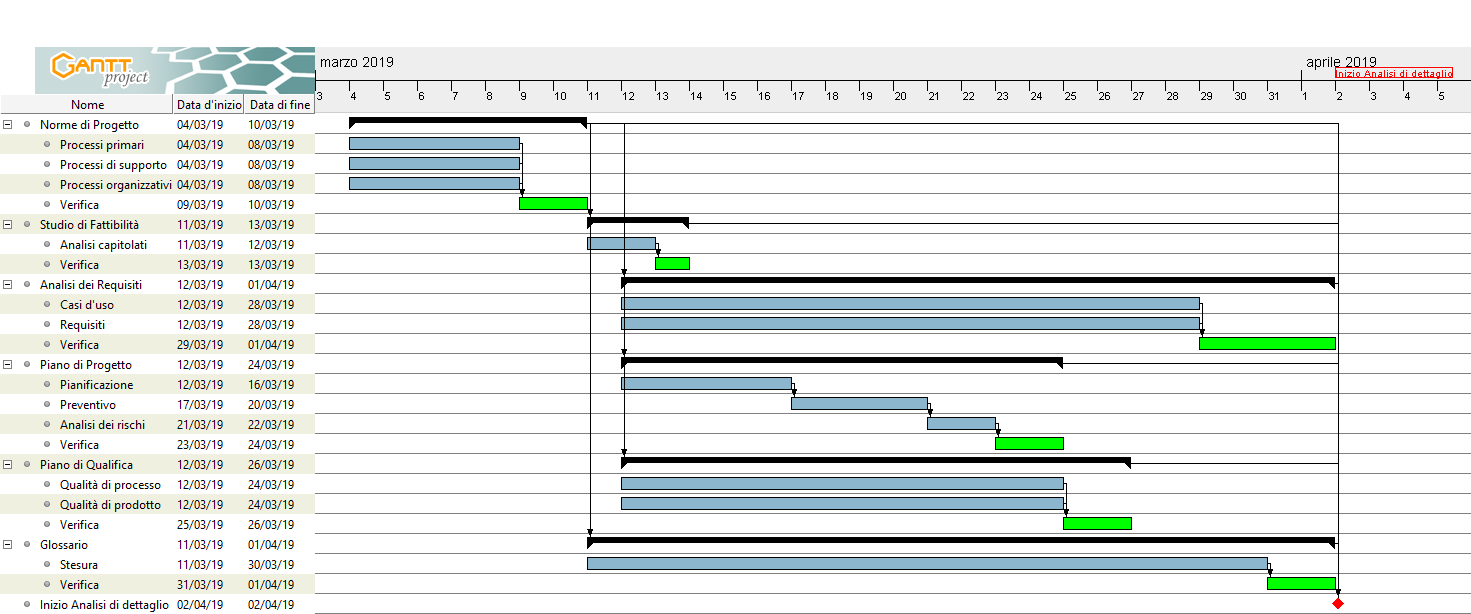
\includegraphics[scale=0.285]{immagini/AnalisiGantt.png}
  \caption{Diagramma di Gantt per la fase di Analisi}
  \end{center}
\end{figure}

\newpage

\subsection{Analisi di dettaglio}
La fase di Analisi di dettaglio ha inizio in data 02-04-2019 e termina il 19-04-2019, data in cui è stata fissata la prima Revisione dei Requisiti e in cui si svolgerà una presentazione del lavoro svolto nelle fasi di Analisi e, in parte, dell'Analisi di Dettaglio. In questo periodo le attività principali consistono nel miglioramento della qualità dei documenti tramite operazioni di incremento e verifica. Particolare attenzione è riservata all'attività di Analisi dei Requisiti che viene ulteriormente sviluppata consolidando i requisiti individuati da parte degli Analisti, successivamente ad incontri con il proponente del progetto. I ruoli attivi in questa fase sono:
\begin{itemize}
    \item \textbf{Responsabile di progetto};
    \item \textbf{Amministratore};
    \item \textbf{Verificatore};
    \item\textbf{Analista}.
\end{itemize}
Oltre all'incremento delle attività contenute nella fase di Analisi vengono aggiunte due nuove attività:
\begin{itemize}
    \item \textbf{Lettera di Presentazione}: Consiste nel redigere una lettera di presentazione, il cui scopo consiste nel presentare il team Cyber13 come fornitore del progetto scelto al proponente;
    \item \textbf{Presentazione}: Consiste nella preparazione dell'attività di presentazione per la Revisione dei Requisiti.
\end{itemize}
Tutte le attività, eccetto quella di Presentazione hanno termine massimo in data 12-04-2019, per cui è prevista la scadenza della consegna del materiale per accesso alla Revisione dei Requisiti.
\subsubsection{Diagramma di Gantt per la fase di Analisi di dettaglio}
\begin{figure}[h!]
\begin{center}
  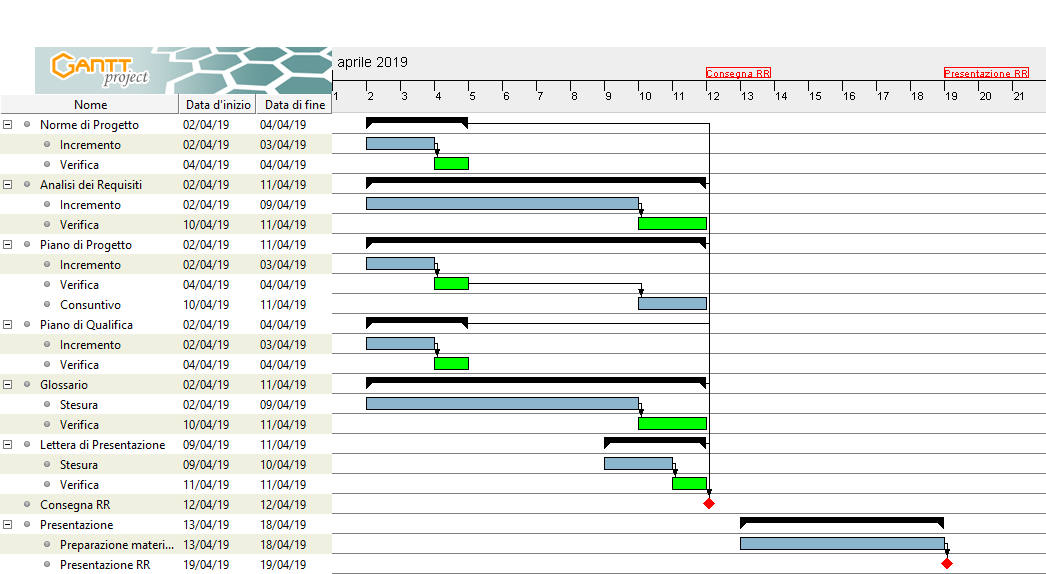
\includegraphics[scale=0.31]{immagini/AnalisiDettaglioGantt.png}
  \caption{Diagramma di Gantt per la fase di Analisi di dettaglio}
  \end{center}
\end{figure}

\newpage 

\subsection{Progettazione della base tecnologica}
La fase di Progettazione della base tecnologica ha inizio in data 20-04-2019 e termina il 17-05-2019. Ha inizio il giorno dopo la presentazione per la Revisione dei Requisiti e si conclude con la presentazione per la Revisione di Progettazione, previa consegna del materiale in data massima 10-05-2019.
I ruoli attivi in questa fase sono:
\begin{itemize}
    \item \textbf{Responsabile di progetto};
    \item \textbf{Amministratore};
    \item \textbf{Progettista};
    \item \textbf{Programmatore};
    \item \textbf{Verificatore};
    \item\textbf{Analista}.
\end{itemize}
Le attività svolte in questa fase sono le seguenti:
\begin{itemize}
    \item \textbf{Incremento e Verifica}: Vengono svolte attività di incremento e verifica sui documenti prodotti nelle fasi precedenti che necessitano di manutenzione per adattarli alle nuove attività (Norme di Progetto, Analisi dei Requisiti, Piano di Progetto, Piano di Qualifica);
    \item \textbf{Technology Baseline}: Consiste nella stesura del documento Technology Baseline da parte dei Progettisti. Tale documento conterrà le scelte progettuali ad alto livello effettuate dal team, oltre alla lista dei framework e delle librerie selezionate per lo sviluppo del prodotto. Questa attività risulta prioritaria durante questa fase dello sviluppo;
    \item \textbf{Proof of Concept}: Consiste nella realizzazione da parte dei programmatori di un piccolo prototipo basato sulle direttive del documento Technology Baseline a prova della validità delle scelte progettuali e tecnologiche effettuate;
    \item \textbf{Glossario}: Consiste nella manutenzione del documento Glossario, che per tutta la durata della fase sarà aggiornato tramite l'aggiunta di nuovi termini dove ritenuto necessario. Comprende anche il miglioramento dei contenuti già presenti;
    \item \textbf{Lettera di Presentazione}: Consiste nel redigere una lettera di presentazione allo scopo di presentare il gruppo per la Revisione di Progettazione;
    \item \textbf{Presentazione}: Consiste nella preparazione dell'attività di presentazione per la Revisione di Progettazione.
\end{itemize}
Tutte le attività, eccetto quella di Presentazione hanno termine massimo in data 10-05-2019, per cui è prevista la scadenza della consegna del materiale per accesso alla Revisione di Progettazione.
\subsubsection{Diagramma di Gantt per la fase di Progettazione della base tecnologica}
\begin{figure}[h!]
\begin{center}
  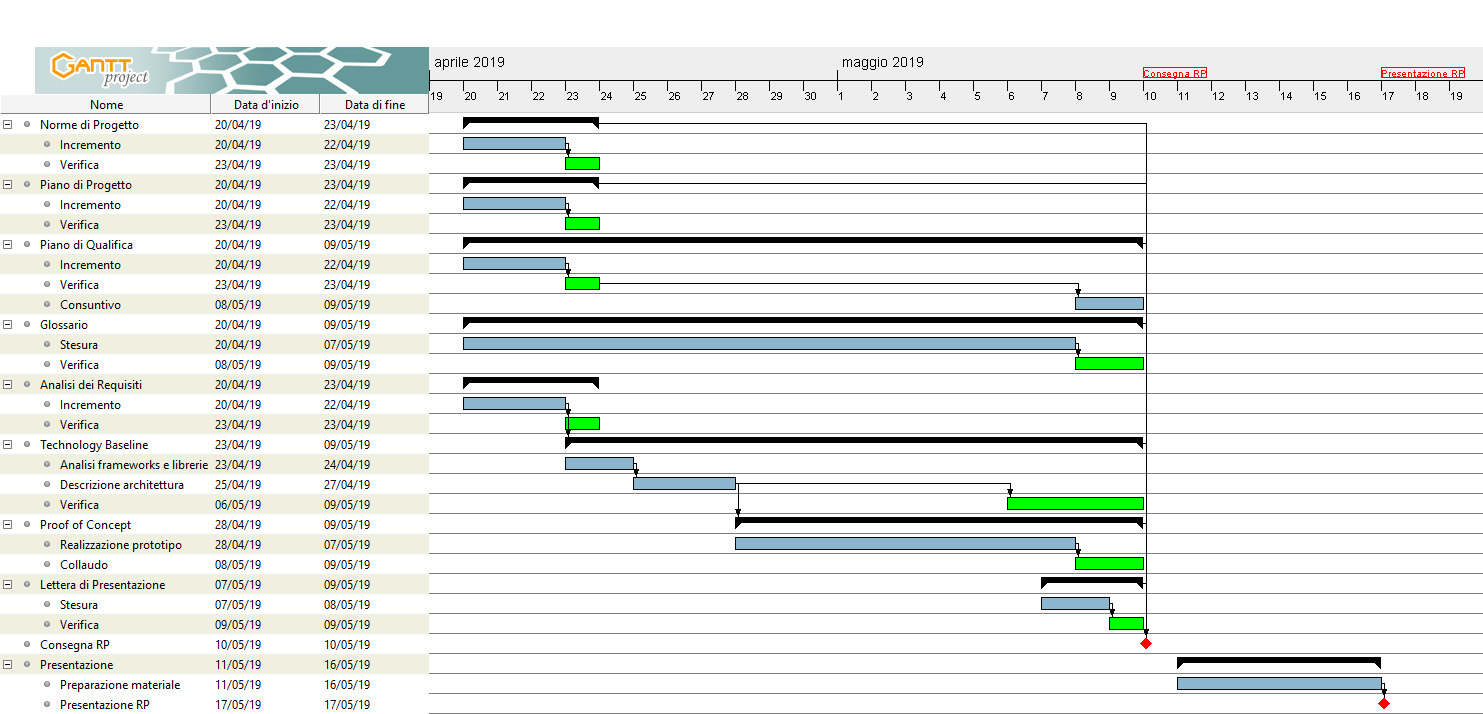
\includegraphics[scale=0.285]{immagini/ProgettazioneGantt.png}
  \caption{Diagramma di Gantt per la fase di Progettazione della base tecnologica}
  \end{center}
\end{figure}

\subsection{Progettazione di dettaglio e codifica}
La fase di Progettazione di dettaglio e codifica ha inizio in data 18-05-2019 e termina il 17-06-2019. Ha inizio il giorno dopo la presentazione per la Revisione di Progetto e si conclude con la presentazione per la Revisione di Qualifica, previa consegna del materiale in data massima 10-06-2019. 
I ruoli attivi in questa fase sono:
\begin{itemize}
    \item \textbf{Responsabile di progetto};
    \item \textbf{Amministratore};
    \item \textbf{Progettista};
    \item \textbf{Programmatore};
    \item \textbf{Verificatore};
    \item\textbf{Analista}.
\end{itemize}
Le attività svolte in questa fase sono le seguenti:
\begin{itemize}
    \item \textbf{Incremento e Verifica}: Vengono svolte attività di incremento e verifica sui documenti prodotti nelle fasi precedenti che necessitano di manutenzione per adattarli alle nuove attività (Norme di Progetto, Piano di Progetto, Piano di Qualifica e Technology Baseline);
    \item \textbf{Product Baseline}: Consiste nella stesura del documento Product Baseline da parte dei Progettisti. Tale documento contiene i dettagli della progettazione architetturale, tramite l'utilizzo di diagrammi delle classi e di sequenza, si deve basare sui contenuti del documento di Technology Baseline;
    \item \textbf{Codifica}: Consiste nella scrittura del codice dell'applicativo e nella sua successiva verifica. Deve basarsi su quanto riportato nel documento di Product Baseline. L'attività è svolta dagli Sviluppatori;
    \item \textbf{Manuale Utente}: Consiste nella stesura del documento Manuale Utente, contenente informazioni sull'utilizzo dell'applicativo prodotto dall'attività di Codifica;
    \item \textbf{Glossario}: Consiste nella manutenzione del documento Glossario, che per tutta la durata della fase sarà aggiornato tramite l'aggiunta di nuovi termini dove ritenuto necessario. Comprende anche il miglioramento dei contenuti già presenti;
    \item \textbf{Lettera di Presentazione}: Consiste nel redigere una lettera di presentazione allo scopo di presentare il gruppo per la Revisione di Qualifica;
    \item \textbf{Presentazione}: Consiste nella preparazione dell'attività di presentazione per la Revisione di Qualifica.
\end{itemize}
Tutte le attività, eccetto quella di Presentazione hanno termine massimo in data 10-06-2019, per cui è prevista la scadenza della consegna del materiale per accesso alla Revisione di Progettazione.
\subsubsection{Diagramma di Gantt per la fase di Progettazione di dettaglio e codifica}
\begin{figure}[h!]
\begin{center}
  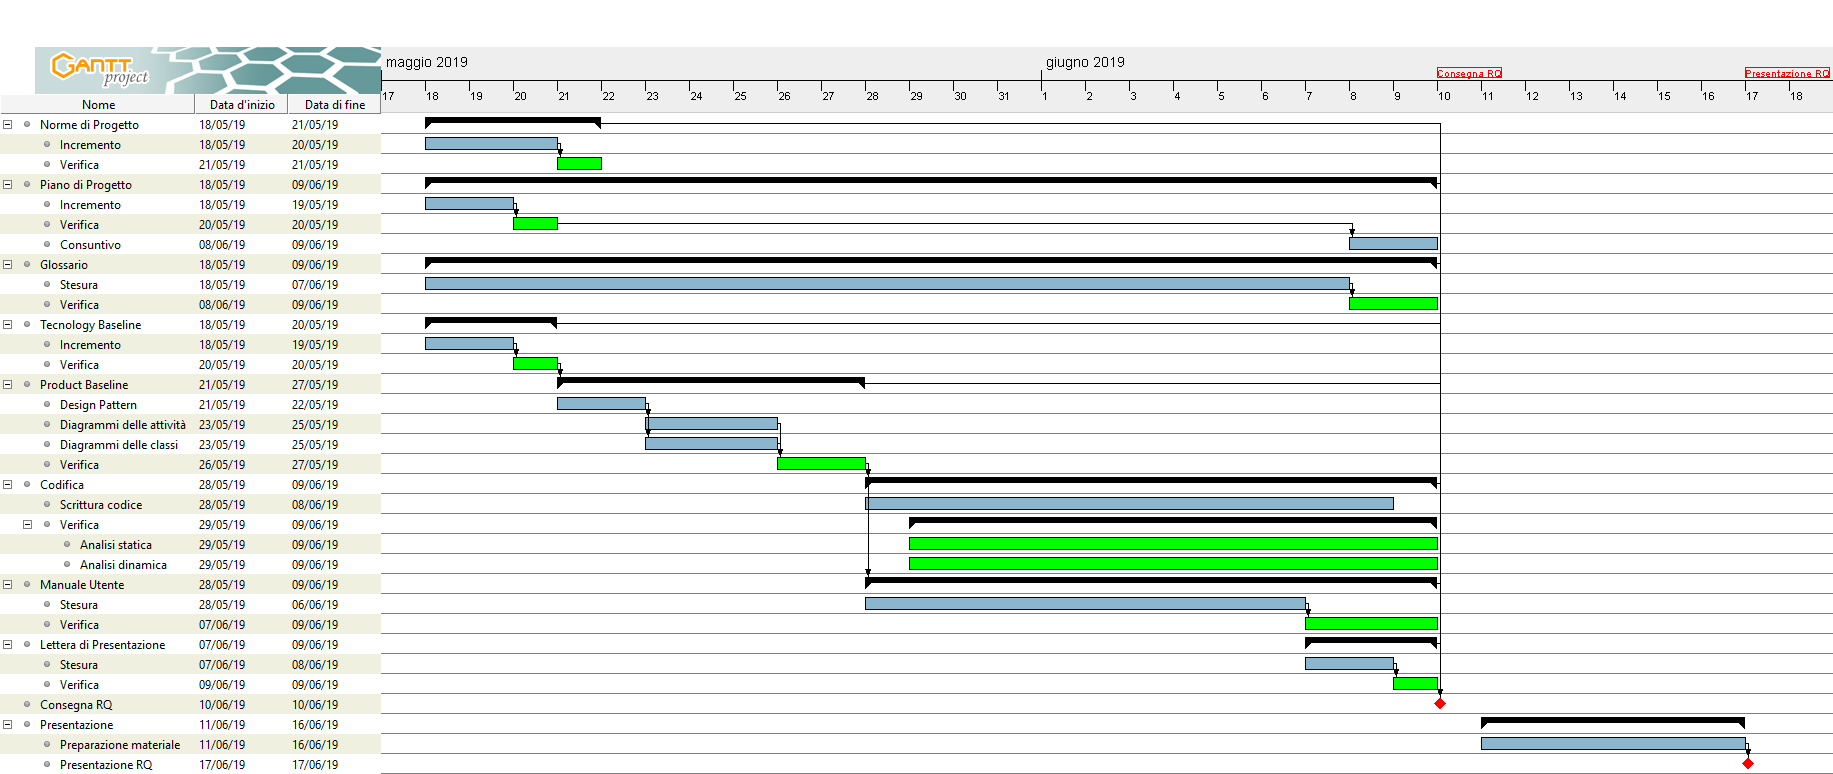
\includegraphics[scale=0.232]{immagini/CodificaGantt.png}
  \caption{Diagramma di Gantt per la fase di Progettazione di dettaglio e codifica}
  \end{center}
\end{figure}

\newpage

\subsection{Validazione e collaudo}
La fase di Progettazione di Validazione e collaudo ha inizio in data 18-06-2019 e termina il 15-07-2019. Ha inizio il giorno dopo la presentazione per la Revisione di Qualifica e si conclude con la presentazione per la Revisione di Accettazione, previa consegna del materiale in data massima 08-06-2019.
I ruoli attivi in questa fase sono:
\begin{itemize}
    \item \textbf{Responsabile di progetto};
    \item \textbf{Amministratore};
    \item \textbf{Progettista};
    \item \textbf{Programmatore};
    \item \textbf{Verificatore}.
\end{itemize}
Le attività svolte in questa fase sono le seguenti:
\begin{itemize}
    \item \textbf{Incremento e Verifica}: Vengono svolte attività di incremento e verifica sui documenti prodotti nelle fasi precedenti che necessitano di manutenzione per adattarli alle nuove attività (Norme di Progetto, Piano di Progetto, Piano di Qualifica, Product Baseline);
    \item \textbf{Validazione}: Consiste nella verifica del software dell'applicativo, effettuata da parte dei Verificatori e Programmatori, per verificare di aver soddisfatto i requisiti individuati nel documento Analisi dei Requisiti e il rispetto delle metriche di qualità presenti nel documento Piano di Qualifica. I programmatori provvedono all'adeguamento del software ai requisiti richiesti;
    \item \textbf{Collaudo}: Consiste nel controllo della correttezza delle funzionalità del prodotto, che viene eseguito e testato in ogni funzionalità richiesta dal proponente. Nell'attività sono coinvolti verificatori e programmatori, al fine di correggere le problematiche nel codice dell'applicativo, se rilevate durante il collaudo;
    \item \textbf{Manuale Utente}: Consiste nel miglioramento e completamento del documento Manuale Utente;
    \item \textbf{Glossario}: Consiste nella manutenzione del documento Glossario, che per tutta la durata della fase sarà aggiornato tramite l'aggiunta di nuovi termini dove ritenuto necessario. Comprende anche il miglioramento dei contenuti già presenti;
    \item \textbf{Lettera di Presentazione}: Consiste nel redigere una lettera di presentazione allo scopo di presentare il prodotto finale alla Revisione di Accettazione;
    \item \textbf{Consegna}: Al termine delle attività di Validazione e Collaudo viene consegnato il prodotto completo, con relativa documentazione, al committente;
    \item \textbf{Presentazione}: Consiste nella preparazione dell'attività di presentazione per la Revisione di Accettazione.
\end{itemize}
Tutte le attività, eccetto quella di Presentazione hanno termine massimo in data 08-07-2019, per cui è prevista la scadenza della consegna del materiale per accesso alla Revisione di Progettazione.
\subsubsection{Diagramma di Gantt per la fase di Validazione e collaudo}

\begin{figure}[h!]
\begin{center}
  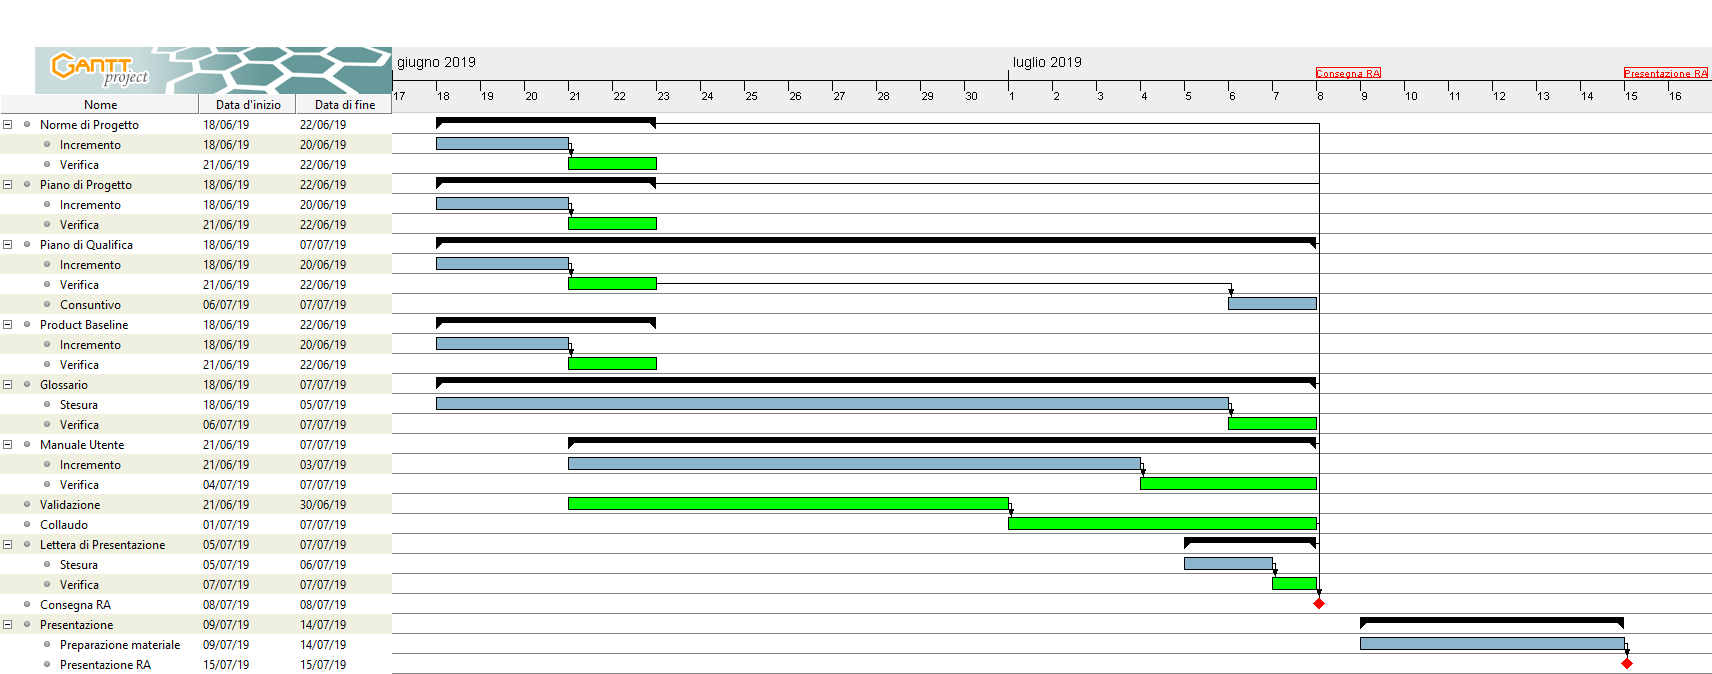
\includegraphics[scale=0.248]{immagini/ValidazioneGantt.png}
  \caption{Diagramma di Gantt per la fase di Validazione e collaudo}
  \end{center}
\end{figure}
    \newpage
        \section{Preventivo}
        Il preventivo che regola la suddivisone oraria delle risorse durante le differenti fasi dello sviluppo tiene in considerazione le seguenti quattro regole principali:
\begin{enumerate}
    \item Ogni membro del gruppo deve ricoprire tutti i ruoli di progetto almeno una volta durante lo sviluppo;
    \item Ogni membro del gruppo dovrà sostenere una quantitativo di lavoro totale rendicontato, non superiore alle 105 ore. Viene considerato rendicontato il lavoro svolto in tutte le fasi dello sviluppo eccetto quelle di Analisi e di Analisi di dettaglio, in quanto le ore dedicate per queste fasi sono considerate di investimento non a carico del committente;
    \item Ogni membro del gruppo dovrà sostenere una mole di lavoro comparabile, le ore di lavoro dovranno essere equamente distribuite in ogni fase dello sviluppo;
    \item Non ci devono essere conflitti interessi tra le attività svolte, in nessun caso un verificatore si deve trovare a dover controllare il proprio lavoro svolto all'interno della stessa fase di sviluppo.
\end{enumerate}
Nelle seguenti tabelle verranno utilizzate le seguenti sigle per indicare i vari ruoli:
\begin{itemize}
    \item \textbf{Re}: Responsabile;
    \item \textbf{Am}: Amministratore;
    \item \textbf{Pj}: Progettista;
    \item \textbf{Pr}: Programmatore;
    \item \textbf{Ve}: Verificatore;
    \item \textbf{An}: Analista.
\end{itemize}
Per facilitare la lettura delle tabelle i valori pari a zero, come quantità di ore, sono stati omessi, lasciando uno spazio vuoto.

\newpage
\subsection{Analisi}
\subsubsection{Prospetto orario}
Nella fase di Analisi la distribuzione oraria dei componenti del gruppo, relativamente ai ruoli da loro assunti, è la seguente:

\begin{table}[H]
\taburowcolors[2] 2{tableLineOne .. tableLineTwo}
\tabulinesep = 10pt
\everyrow{\tabucline[.4mm  white]{}}
\begin{tabu} to \textwidth { X[c,4] X[c] X[c] X[c] X[c] X[c] X[c] X[c,2]}
    \tableHeaderStyle
    Nome & Re & Am &  Pj & Pr & Ve & An & Totale \\
    Daniel Mirel Bira &  & 10 &   &  &  & 12 & 22 \\
    Andrea Casagrande &  & 4 &   &  & 12 & 7 & 23 \\
    Fabio Garavello &  & 8 &   &  & 15 &  & 23 \\
    Elena Pontecchiani & 12 & 4 &   &  &  & 7 & 23 \\
    Ilaria Rizzo &  & 3 &   &  & 4 & 15 & 22 \\
    Matteo Squeri & 13 &  &   &  & 7 & 3 & 23 \\
\end{tabu}
\caption{Prospetto orario - Analisi}
\end{table}

Il seguente grafico dà una rappresentazione visiva della suddivisione oraria: 

\begin{figure}[h!]
  \begin{center}
  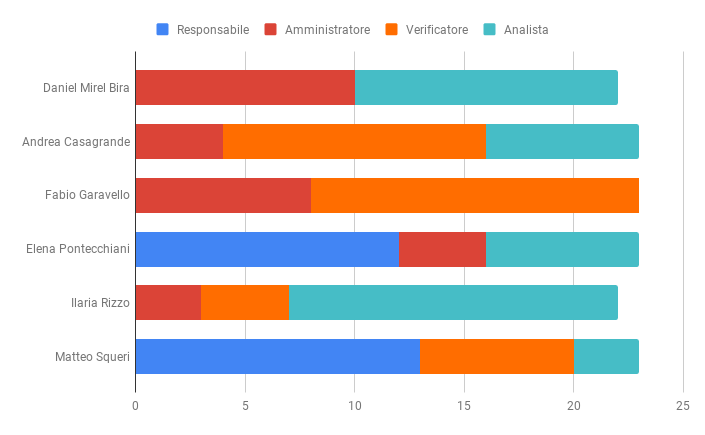
\includegraphics[scale=0.50]{immagini/AnalisiG.png}
  \caption{Grafico suddivisione oraria della fase di Analisi}
  \end{center}
\end{figure}

\newpage
\subsubsection{Prospetto economico}
Nella fase di Analisi la distribuzione delle ore tra i differenti ruoli, con relativo costo, è la seguente:

\begin{table}[H]
\taburowcolors[2] 2{tableLineOne .. tableLineTwo}
\tabulinesep = 10pt
\everyrow{\tabucline[.4mm  white]{}}
\begin{tabu} to \textwidth { X[c] X[c] X[c] }
    \tableHeaderStyle
    Ruolo & Ore & Costo in \euro \\
    Responsabile & 25 & 750,00 \\
    Amministratore & 29 & 580,00 \\
    Progettista &  &  \\
    Programmatore &  &  \\
    Verificatore & 38 & 570,00 \\
    Analista & 44 & 1.100,00 \\
    \textbf{Totale} & \textbf{136} & \textbf{3.000,00} \\
\end{tabu}
\caption{Prospetto economico - Analisi}
\end{table}

Il seguente grafico dà una rappresentazione visiva della suddivisione dei ruoli:

\begin{figure}[h!]
\begin{center}
  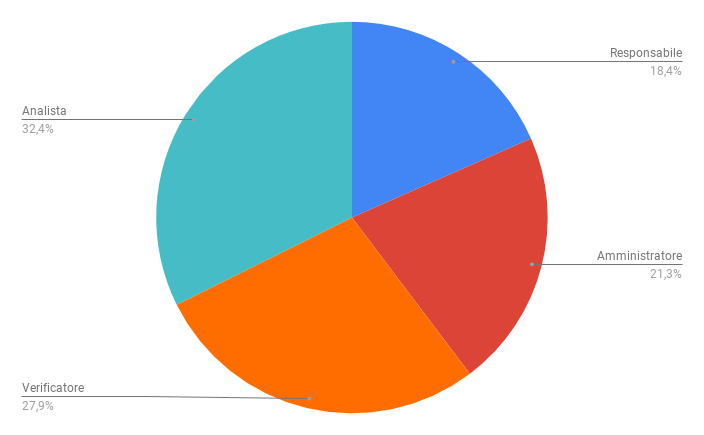
\includegraphics[scale=0.50]{immagini/AnalisiRG.png}
  \caption{Grafico suddivisione dei ruoli della fase di Analisi}
  \end{center}
\end{figure}

\newpage
\subsection{Analisi di dettaglio}
\subsubsection{Prospetto orario}
Nella fase di Analisi di dettaglio la distribuzione oraria dei componenti del gruppo, relativamente ai ruoli da loro assunti, è la seguente:

\begin{table}[H]
\taburowcolors[2] 2{tableLineOne .. tableLineTwo}
\tabulinesep = 10pt
\everyrow{\tabucline[.4mm  white]{}}
\begin{tabu} to \textwidth { X[c,4] X[c] X[c] X[c] X[c] X[c] X[c] X[c,2]}
    \tableHeaderStyle
    Nome & Re & Am &  Pj & Pr & Ve & An & Totale \\
    Daniel Mirel Bira &  &  &   &  & 5 & 3 & 8 \\
    Andrea Casagrande & 7 &  &   &  &  &  & 7 \\
    Fabio Garavello &  & 2 &   &  &  & 6 & 8 \\
    Elena Pontecchiani &  & 4 &   &  &  & 4 & 8 \\
    Ilaria Rizzo &  &  &   &  & 7 &  & 7 \\
    Matteo Squeri &  & 3 &   &  &  & 4 & 7 \\
\end{tabu}
\caption{Prospetto orario - Analisi di dettaglio}
\end{table}

Il seguente grafico dà una rappresentazione visiva della suddivisione oraria:

\begin{figure}[h!]
  \begin{center}
  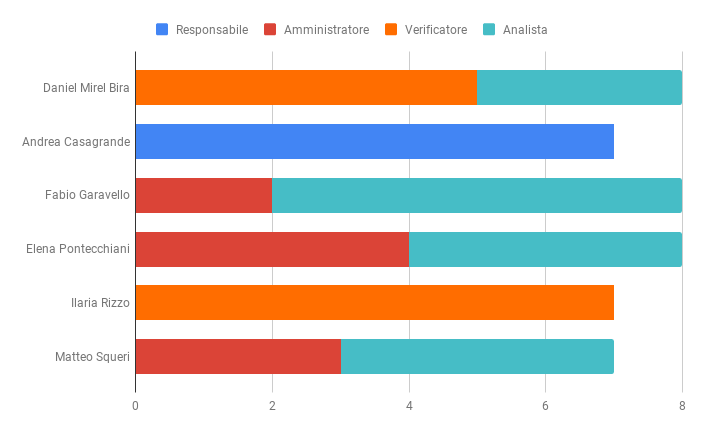
\includegraphics[scale=0.50]{immagini/DettaglioG.png}
  \caption{Grafico suddivisione oraria della fase di Analisi di dettaglio}
  \end{center}
\end{figure}

\newpage
\subsubsection{Prospetto economico}
Nella fase di Analisi di dettaglio la distribuzione delle ore tra i differenti ruoli, con relativo costo, è la seguente:

\begin{table}[H]
\taburowcolors[2] 2{tableLineOne .. tableLineTwo}
\tabulinesep = 10pt
\everyrow{\tabucline[.4mm  white]{}}
\begin{tabu} to \textwidth { X[c] X[c] X[c] }
    \tableHeaderStyle
    Ruolo & Ore & Costo in \euro \\
    Responsabile & 7 & 210,00 \\
    Amministratore & 9 & 180,00 \\
    Progettista &  &  \\
    Programmatore &  &  \\
    Verificatore & 12 & 180,00 \\
    Analista & 17 & 425,00 \\
    \textbf{Totale} & \textbf{45} & \textbf{995,00} \\
\end{tabu}
\caption{Prospetto economico - Analisi di dettaglio}
\end{table}

Il seguente grafico dà una rappresentazione visiva della suddivisione dei ruoli:

\begin{figure}[h!]
  \begin{center}
  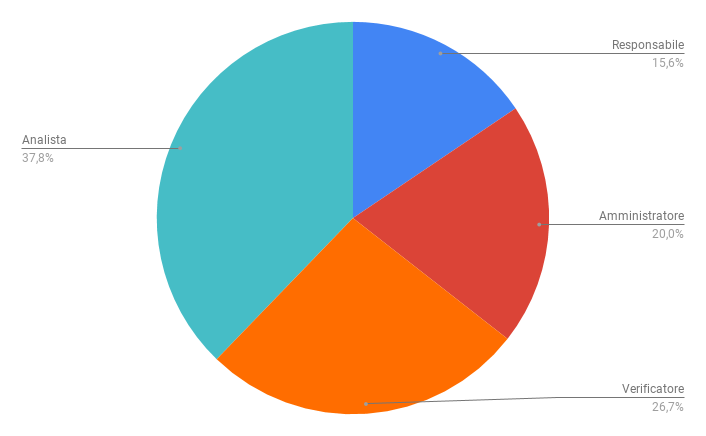
\includegraphics[scale=0.50]{immagini/DettaglioRG.png}
  \caption{Grafico suddivisione dei ruoli della fase di Analisi di dettaglio}
  \end{center}
\end{figure}

\newpage
\subsection{Progettazione della base tecnologica}
\subsubsection{Prospetto orario}
Nella fase di Progettazione della base tecnologica la distribuzione oraria dei componenti del gruppo, relativamente ai ruoli da loro assunti, è la seguente:

\begin{table}[H]
\taburowcolors[2] 2{tableLineOne .. tableLineTwo}
\tabulinesep = 10pt
\everyrow{\tabucline[.4mm  white]{}}
\begin{tabu} to \textwidth { X[c,4] X[c] X[c] X[c] X[c] X[c] X[c] X[c,2]}
    \tableHeaderStyle
    Nome & Re & Am &  Pj & Pr & Ve & An & Totale \\
    Daniel Mirel Bira & 5 &  &   & 18 & 12 &  & 35 \\
    Andrea Casagrande &  & 8 & 15  & 7 & 4 &  & 34 \\
    Fabio Garavello & 5 &  & 6  & 7 & 10 & 7 & 35 \\
    Elena Pontecchiani &  &  & 8  & 8 & 14 & 5 & 35 \\
    Ilaria Rizzo &  & 4 &  10 & 15 & 6 &  & 35 \\
    Matteo Squeri &  &  & 13 & 6 & 5 & 10 & 34 \\
\end{tabu}
\caption{Prospetto orario - Progettazione della base tecnologica}
\end{table}

Il seguente grafico dà una rappresentazione visiva della suddivisione oraria:

\begin{figure}[h!]
  \begin{center}
  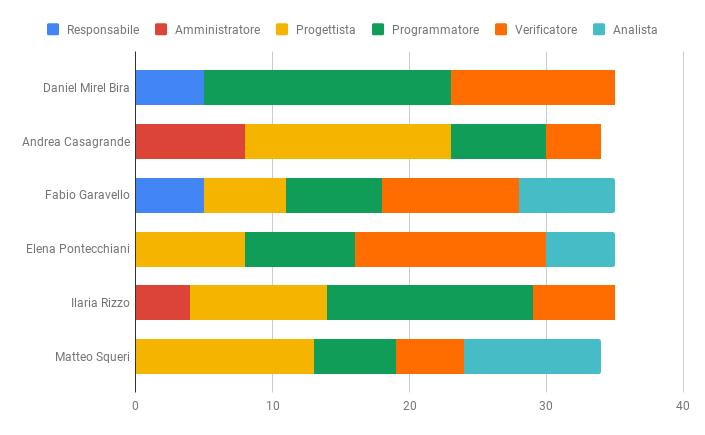
\includegraphics[scale=0.50]{immagini/ProgettazioneG.png}
  \caption{Grafico suddivisione oraria della fase di Progettazione della base tecnologica}
  \end{center}
\end{figure}

\newpage
\subsubsection{Prospetto economico}
Nella fase di Progettazione della base tecnologica la distribuzione delle ore tra i differenti ruoli, con relativo costo, è la seguente:

\begin{table}[H]
\taburowcolors[2] 2{tableLineOne .. tableLineTwo}
\tabulinesep = 10pt
\everyrow{\tabucline[.4mm  white]{}}
\begin{tabu} to \textwidth { X[c] X[c] X[c] }
    \tableHeaderStyle
    Ruolo & Ore & Costo in \euro \\
    Responsabile & 10 & 300,00  \\
    Amministratore & 12 & 240,00 \\
    Progettista & 52 & 1.144,00 \\
    Programmatore & 61 & 915,00 \\
    Verificatore & 51 & 765,00 \\
    Analista & 22 & 550,00 \\
    \textbf{Totale} & \textbf{208} & \textbf{3.914,00} \\
\end{tabu}
\caption{Prospetto economico - Progettazione della base tecnologica}
\end{table}

Il seguente grafico dà una rappresentazione visiva della suddivisione dei ruoli:

\begin{figure}[h!]
  \begin{center}
  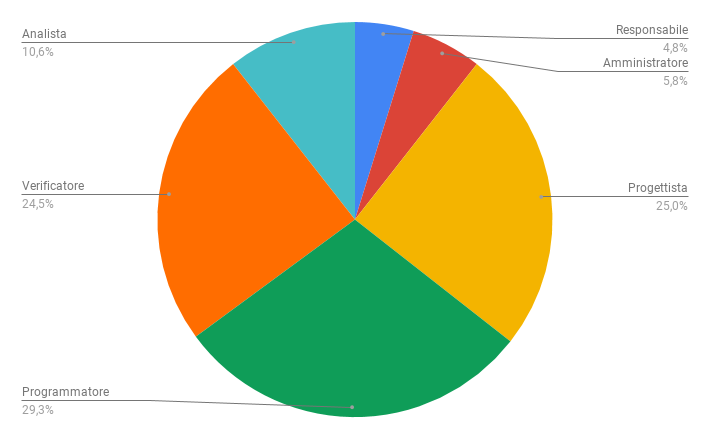
\includegraphics[scale=0.50]{immagini/ProgettazioneRG.png}
  \caption{Grafico suddivisione dei ruoli della fase di Progettazione della base tecnologica}
  \end{center}
\end{figure}

\newpage
\subsection{Progettazione di dettaglio e codifica}
\subsubsection{Prospetto orario}
Nella fase di Progettazione di dettaglio e codifica la distribuzione oraria dei componenti del gruppo, relativamente ai ruoli da loro assunti, è la seguente:

\begin{table}[H]
\taburowcolors[2] 2{tableLineOne .. tableLineTwo}
\tabulinesep = 10pt
\everyrow{\tabucline[.4mm  white]{}}
\begin{tabu} to \textwidth { X[c,4] X[c] X[c] X[c] X[c] X[c] X[c] X[c,2]}
    \tableHeaderStyle
    Nome & Re & Am &  Pj & Pr & Ve & An & Totale \\
    Daniel Mirel Bira &  &  & 20 & 25 &  &  & 45 \\
    Andrea Casagrande &  &  & 13 & 16 & 14 & 2 & 45 \\
    Fabio Garavello &  & 5 &  8 & 15 & 12 & 5 & 45 \\
    Elena Pontecchiani &  & 5 &  12 & 17 & 10  &  & 44  \\
    Ilaria Rizzo & 10 &  &  8 & 18 & 8 &  & 44 \\
    Matteo Squeri & 3 &  & 12 & 20 & 10 &  & 45 \\
\end{tabu}
\caption{Prospetto orario - Progettazione di dettaglio e codifica}
\end{table}

Il seguente grafico dà una rappresentazione visiva della suddivisione oraria:

\begin{figure}[h!]
  \begin{center}
  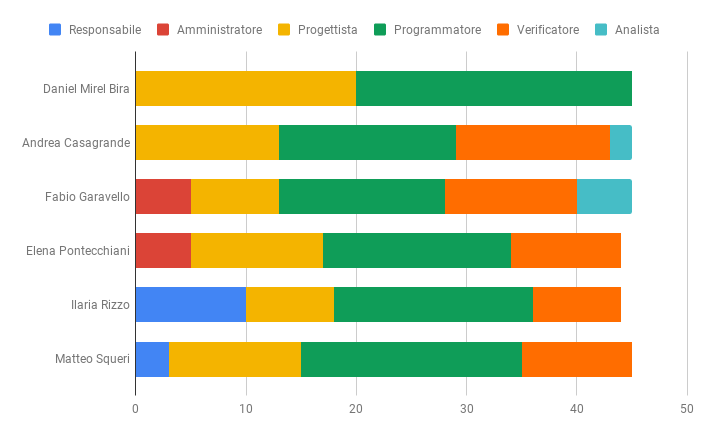
\includegraphics[scale=0.50]{immagini/CodingG.png}
  \caption{Grafico suddivisione oraria della fase di Progettazione di dettaglio e codifica}
  \end{center}
\end{figure}

\newpage
\subsubsection{Prospetto economico}
Nella fase di Progettazione di dettaglio e codifica la distribuzione delle ore tra i differenti ruoli, con relativo costo, è la seguente:

\begin{table}[H]
\taburowcolors[2] 2{tableLineOne .. tableLineTwo}
\tabulinesep = 10pt
\everyrow{\tabucline[.4mm  white]{}}
\begin{tabu} to \textwidth { X[c] X[c] X[c] }
    \tableHeaderStyle
    Ruolo & Ore & Costo in \euro \\
    Responsabile & 13 & 390,00 \\
    Amministratore & 10 & 200,00 \\
    Progettista & 73 & 1.606,00 \\
    Programmatore & 111 & 1.665,00 \\
    Verificatore & 54 & 810,00 \\
    Analista & 7 & 175,00 \\
    \textbf{Totale} & \textbf{268} & \textbf{4.846,00} \\
\end{tabu}
\caption{Prospetto economico - Progettazione di dettaglio e codifica}
\end{table}

Il seguente grafico dà una rappresentazione visiva della suddivisione dei ruoli:

\begin{figure}[h!]
  \begin{center}
  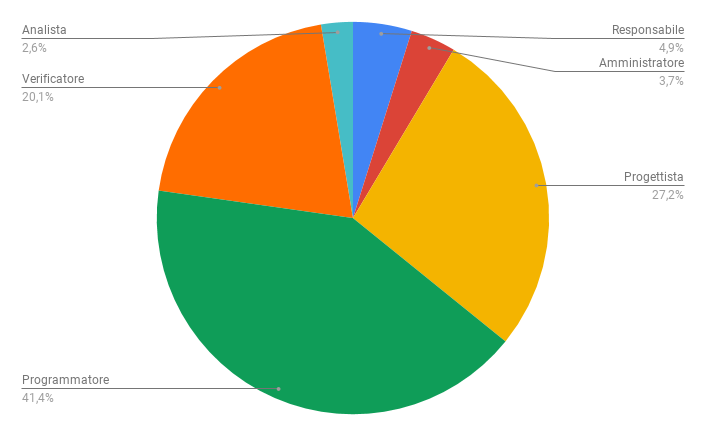
\includegraphics[scale=0.50]{immagini/CodingRG.png}
  \caption{Grafico suddivisione dei ruoli della fase di Progettazione di dettaglio e codifica}
  \end{center}
\end{figure}

\newpage
\subsection{Validazione e collaudo}
\subsubsection{Prospetto orario}
Nella fase di Validazione e collaudo la distribuzione oraria dei componenti del gruppo, relativamente ai ruoli da loro assunti, è la seguente:

\begin{table}[H]
\taburowcolors[2] 2{tableLineOne .. tableLineTwo}
\tabulinesep = 10pt
\everyrow{\tabucline[.4mm  white]{}}
\begin{tabu} to \textwidth { X[c,4] X[c] X[c] X[c] X[c] X[c] X[c] X[c,2]}
    \tableHeaderStyle
    Nome & Re & Am &  Pj & Pr & Ve & An & Totale \\
    Daniel Mirel Bira &  &  &  & 8 & 15 &  & 23 \\
    Andrea Casagrande & 12 & 4 &  &  & 8 &  & 24 \\
    Fabio Garavello &  &  &  10 & 5 & 8 &  & 23 \\
    Elena Pontecchiani &  &  &   & 12 & 12  &  & 24  \\
    Ilaria Rizzo & 4 & 2 & 4 & 10 & 4 &  & 24 \\
    Matteo Squeri &  & 10 & 6 &  & 8 &  & 24\\
\end{tabu}
\caption{Prospetto orario - Validazione e collaudo}
\end{table}

Il seguente grafico dà una rappresentazione visiva della suddivisione oraria:

\begin{figure}[h!]
  \begin{center}
  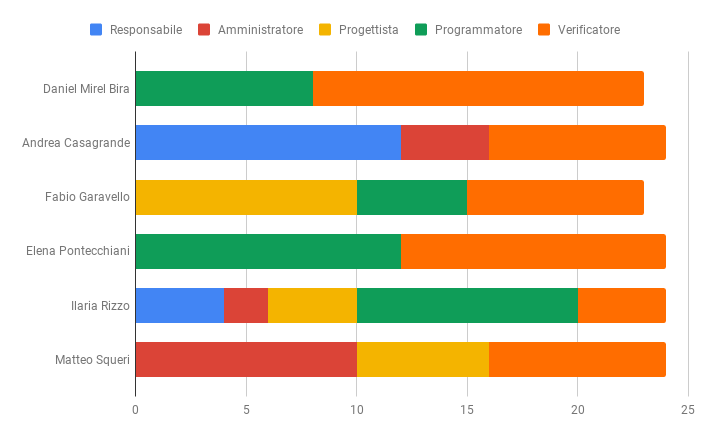
\includegraphics[scale=0.50]{immagini/VerificaG.png}
  \caption{Grafico suddivisione oraria della fase di Validazione e collaudo}
  \end{center}
\end{figure}

\newpage
\subsubsection{Prospetto economico}
Nella fase di Validazione e collaudo la distribuzione delle ore tra i differenti ruoli, con relativo costo, è la seguente:

\begin{table}[H]
\taburowcolors[2] 2{tableLineOne .. tableLineTwo}
\tabulinesep = 10pt
\everyrow{\tabucline[.4mm  white]{}}
\begin{tabu} to \textwidth { X[c] X[c] X[c] }
    \tableHeaderStyle
    Ruolo & Ore & Costo in \euro \\
    Responsabile & 16 & 480,00 \\
    Amministratore & 16  & 320,00 \\
    Progettista & 20 & 440,00 \\
    Programmatore & 35 & 525,00 \\
    Verificatore & 55 & 825,00 \\
    Analista &  &  \\
    \textbf{Totale} & \textbf{142} & \textbf{2.590,00} \\
\end{tabu}
\caption{Prospetto economico - Validazione e collaudo}
\end{table}

Il seguente grafico dà una rappresentazione visiva della suddivisione dei ruoli:

\begin{figure}[h!]
  \begin{center}
  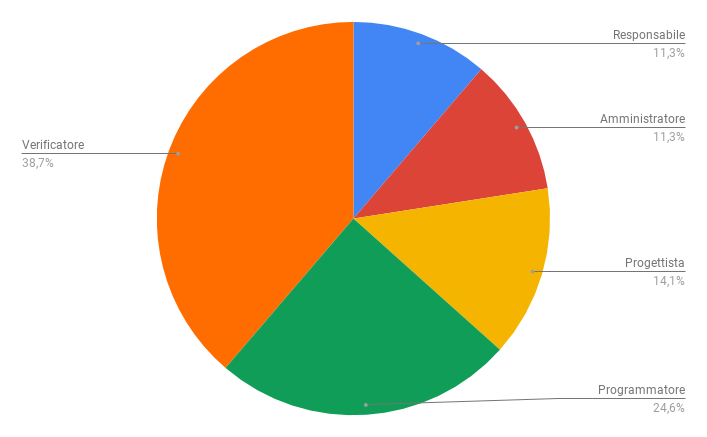
\includegraphics[scale=0.50]{immagini/VerificaRG.png}
  \caption{Grafico suddivisione dei ruoli della fase di Validazione e collaudo}
  \end{center}
\end{figure}

\newpage
\subsection{Totale ore rendicontate}
\subsubsection{Totale suddivisione ore rendicontate}
Sono riportate in questa sezione il totale delle ore di lavoro di ciascun membro del gruppo a carico del \citgl{committente}. Non sono comprese le ore preventivate per le fasi di Analisi e Analisi di dettaglio in quanto considerate di investimento e formazione e quindi non rendicontabili.

\begin{table}[H]
\taburowcolors[2] 2{tableLineOne .. tableLineTwo}
\tabulinesep = 10pt
\everyrow{\tabucline[.4mm  white]{}}
\begin{tabu} to \textwidth { X[c,4] X[c] X[c] X[c] X[c] X[c] X[c] X[c,2]}
    \tableHeaderStyle
    Nome & Re & Am &  Pj & Pr & Ve & An & Totale \\
    Daniel Mirel Bira & 5 &  & 20 & 51 & 27 &  & 103 \\
    Andrea Casagrande & 12 & 12 & 28 & 23 & 26 & 2 & 103 \\
    Fabio Garavello & 5 & 5 & 24 & 27 & 30 & 12 & 103 \\
    Elena Pontecchiani &  & 5 & 20  & 37 & 36  & 5 & 103  \\
    Ilaria Rizzo & 14 & 6 & 22 & 43 & 18 &  & 103 \\
    Matteo Squeri & 3 & 10 & 31 & 26 & 23 & 10 & 103 \\
\end{tabu}
\caption{Totale suddivisione delle ore rendicontate}
\end{table}

Il seguente grafico dà una rappresentazione visiva della suddivisione oraria:

\begin{figure}[h!]
  \begin{center}
  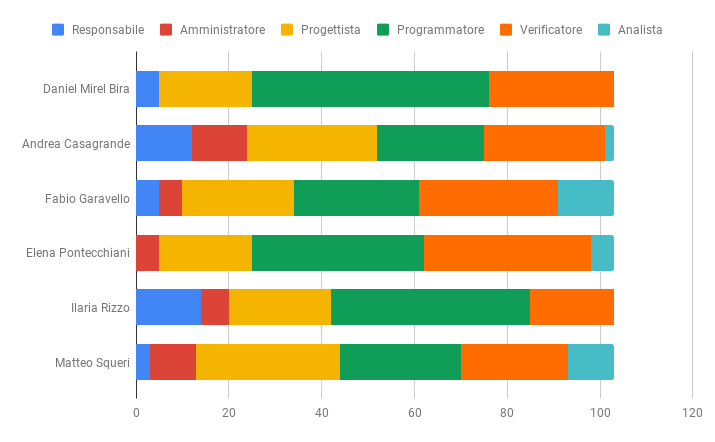
\includegraphics[scale=0.50]{immagini/RendicontateG.png}
  \caption{Grafico della totale suddivisione oraria delle ore rendicontate}
  \end{center}
\end{figure}

\newpage
\subsubsection{Totale del prospetto economico rendicontato}
Sono riportati in questa sezione il costo totale di ogni ruolo, in relazione alle ore in cui sarà attivo, considerando solo le fasi in cui le ore di lavoro sono a carico del committente. Non sono quindi compresi i costi preventivati per le fasi di Analisi e Analisi di dettaglio.

\begin{table}[H]
\taburowcolors[2] 2{tableLineOne .. tableLineTwo}
\tabulinesep = 10pt
\everyrow{\tabucline[.4mm  white]{}}
\begin{tabu} to \textwidth { X[c] X[c] X[c] }
    \tableHeaderStyle
    Ruolo & Ore & Costo in \euro \\
    Responsabile & 39 & 1.170,00 \\
    Amministratore & 38 & 760,00 \\
    Progettista & 145 & 3.190,00 \\
    Programmatore & 207 & 3.105,00 \\
    Verificatore & 160 & 2.400,00 \\
    Analista & 29 & 725,00 \\
    \textbf{Totale} & \textbf{618} & \textbf{11.350,00} \\
\end{tabu}
\caption{Totale del prospetto economico rendicontato}
\end{table}

Il seguente grafico dà una rappresentazione visiva della suddivisione dei ruoli:

\begin{figure}[h!]
  \begin{center}
  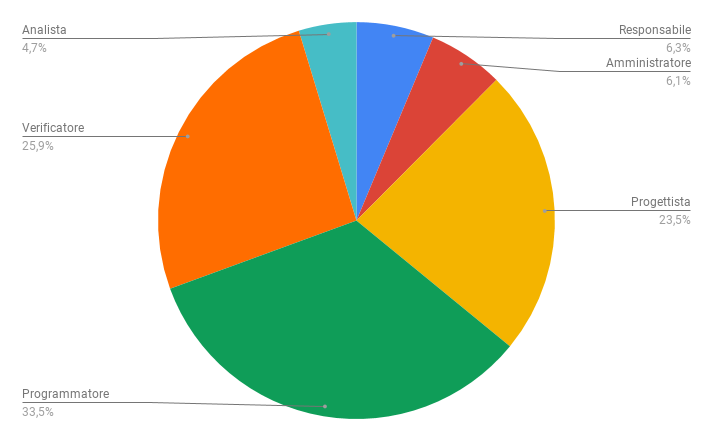
\includegraphics[scale=0.45]{immagini/RendicontateRG.png}
  \caption{Grafico della totale suddivisione dei ruoli delle ore rendicontate}
  \end{center}
\end{figure}

\newpage
\subsection{Totale ore con investimento}
\subsubsection{Totale suddivisione ore con investimento}
Sono riportate in questa sezione il totale delle ore di lavoro preventivate per ciascun membro considerando ogni fase del progetto. 

\begin{table}[H]
\taburowcolors[2] 2{tableLineOne .. tableLineTwo}
\tabulinesep = 10pt
\everyrow{\tabucline[.4mm  white]{}}
\begin{tabu} to \textwidth { X[c,4] X[c] X[c] X[c] X[c] X[c] X[c] X[c,2]}
    \tableHeaderStyle
    Nome & Re & Am &  Pj & Pr & Ve & An & Totale \\
    Daniel Mirel Bira & 5 & 10 & 20 & 51 & 32 & 15 & 133 \\
    Andrea Casagrande & 19 & 16 & 28 & 23 & 38 & 9 & 133 \\
    Fabio Garavello & 5 & 15 & 24 & 27 & 45 & 18 & 134 \\
    Elena Pontecchiani & 12 & 13 & 20 & 37 & 36  & 16 & 134  \\
    Ilaria Rizzo & 14 & 9 & 22 & 43 & 29 & 15 & 132 \\
    Matteo Squeri & 16 & 13 & 31 & 26 & 30 & 17 & 133 \\
\end{tabu}
\caption{Totale suddivisione delle ore con investimento}
\end{table}

Il seguente grafico dà una rappresentazione visiva della suddivisione oraria:

\begin{figure}[h!]
  \begin{center}
  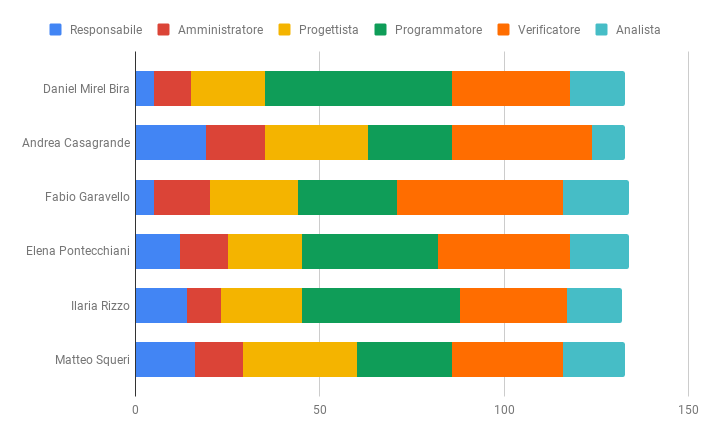
\includegraphics[scale=0.50]{immagini/InvestimentoG.png}
  \caption{Grafico della totale suddivisione oraria delle ore con investimento}
  \end{center}
\end{figure}

\newpage
\subsubsection{Totale del prospetto economico con investimento}
Sono riportati in questa sezione il costo totale di ogni ruolo, in relazione alle ore in cui sarà attivo, considerando ogni fase del progetto.

\begin{table}[H]
\taburowcolors[2] 2{tableLineOne .. tableLineTwo}
\tabulinesep = 10pt
\everyrow{\tabucline[.4mm  white]{}}
\begin{tabu} to \textwidth { X[c] X[c] X[c] }
    \tableHeaderStyle
    Ruolo & Ore & Costo in \euro \\
    Responsabile & 71 & 2.130,00 \\
    Amministratore & 76 & 1.520,00 \\
    Progettista & 145 & 3.190,00 \\
    Programmatore & 207 & 3.105,00 \\
    Verificatore & 210 & 3.150,00 \\
    Analista & 90 & 2.250,00 \\
    \textbf{Totale} & \textbf{799} & \textbf{15.345,00} \\
\end{tabu}
\caption{Totale del prospetto economico con investimento}
\end{table}

Il seguente grafico dà una rappresentazione visiva della suddivisione dei ruoli:

\begin{figure}[h!]
  \begin{center}
  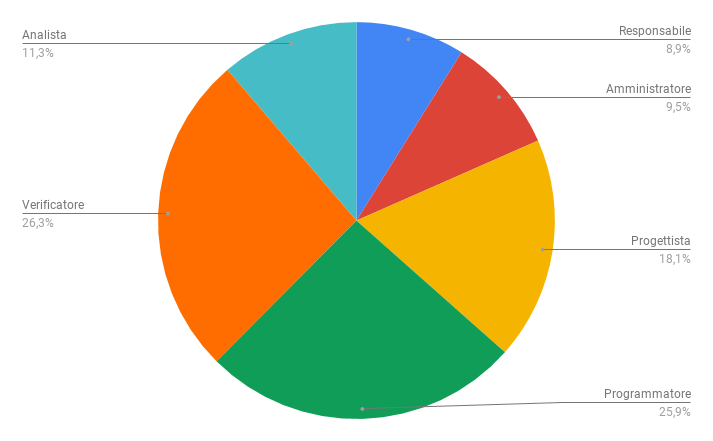
\includegraphics[scale=0.45]{immagini/InvestimentoRG.png}
  \caption{Grafico della totale suddivisione dei ruoli delle ore con investimento}
  \end{center}
\end{figure}
    \newpage
        \section{Consultivo e preventivo a finire}
        \subsection{Consuntivo e preventivo a finire}
In questa sezioni verranno riportati i consuntivi delle varie fasi con delle conclusioni sullo stato dello sviluppo. Viene inoltre allegato un preventivo a finire che terrà conto delle sole fasi le cui ore vengono rendicontate. \\
Nei consuntivi vengono riportati:
\begin{itemize}
    \item le ore e i costi preventivati;
    \item le ore e i costi effettivi;
\end{itemize}l
Viene inserito tra parentesi, a fianco dei costi e delle ore effettive, un valore che rappresenta la differenza rispetto a quanto preventivato:  
\begin{itemize}
    \item \textbf{Positivo}: Se le ore effettive sono minori rispetto a quelle preventivate o se il costo è diminuito.
    \item \textbf{Negativo}: Se le ore effettive sono maggiori rispetto a quelle preventivate o se il costo è aumentato.
\end{itemize}
Se non sono presenti valori tra parentesi significa che il numero di ore e i costi per i ruoli sono state come preventivate.
\subsubsection{Consuntivi fasi di Analisi e Analisi di dettaglio}
Essendo entrambe le fasi precedenti alla Revisione dei Requisiti, vengono considerate assieme. La consegna del materiale è fissata in data 12-04-2019, durante la fase di Analisi di dettaglio, è seguita poi dalla sola preparazione della presentazione, la quale non comporta l'impiego di specifici ruoli con conseguenti costi economici, perciò il consuntivo non tiene conto del periodo che va dal 13-04-2019 al 19-04-2019.

\newpage

\paragraph{Consuntivo fase di Analisi}
La seguente tabella contiene i dati sia orari che economici del consuntivo per la fase di Analisi:

\begin{table}[H]
\taburowcolors[2] 2{tableLineOne .. tableLineTwo}
\tabulinesep = 10pt
\everyrow{\tabucline[.4mm  white]{}}
\begin{tabu} to \textwidth { X[c,1.2] X[c] X[c] X[c,1.1] X[c]}
    \tableHeaderStyle
    Ruolo & Ore preventivate & Ore effettive & Costi preventivati in \euro & Costi effettivi in \euro \\
    Responsabile & 25 & 22 (+3) & 720,00 & 630,00 (+90)\\
    Amministratore & 29 & 25 (+4) & 580,00 & 500,00 (+80)\\
    Progettista &  &  &  & \\
    Programmatore &  &  &  & \\
    Verificatore & 38 & 35 (+3) & 570,00 & 525 (+45)\\
    Analista & 44 & 50 (-6) & 1.100,00 & 1.250,00 (-150) \\
    \textbf{Totale} & \textbf{136} & \textbf{132 (+4)} & \textbf{3.000,00} & \textbf{2.905,00 (+95)}  \\
\end{tabu}
\caption{Consuntivo fase di Analisi}
\end{table}
Resoconto:
\begin{itemize}
    \item \textbf{Differenza oraria}: +4 ore;
    \item \textbf{Differenza costi}: +95 \euro ;
\end{itemize}
Non sono stati commessi dei ritardi durante l’esecuzione delle varie attività previste.

\newpage

\paragraph{Consuntivo fase di Analisi di dettaglio}
La seguente tabella contiene i dati sia orari che economici del consuntivo per la fase di Analisi di dettaglio:

\begin{table}[H]
\taburowcolors[2] 2{tableLineOne .. tableLineTwo}
\tabulinesep = 10pt
\everyrow{\tabucline[.4mm  white]{}}
\begin{tabu} to \textwidth { X[c,1.2] X[c] X[c] X[c,1.1] X[c]}
    \tableHeaderStyle
    Ruolo & Ore preventivate & Ore effettive & Costi preventivati in \euro & Costi effettivi in \euro \\
    Responsabile & 7 & 7 & 210,00 & 210,00\\
    Amministratore & 9 & 6 (+3) & 180,00 &  120,00 (+60)\\
    Progettista &  &  &  & \\
    Programmatore &  &  &  & \\
    Verificatore & 12 & 20 (-8) & 180,00 & 300,00 (-120,00)\\
    Analista & 17 & 11 (+6) & 425,00 & 275,00 (+150)  \\
    \textbf{Totale} & \textbf{45} & \textbf{44 (+1)} & \textbf{995,00} & \textbf{905,00 (+90)}  \\
\end{tabu}
\caption{Consuntivo fase di Analisi di dettaglio}
\end{table}
Resoconto:
\begin{itemize}
    \item \textbf{Differenza oraria}: +1 ore;
    \item \textbf{Differenza costi}: +90 \euro ;
\end{itemize}
Non sono stati commessi dei ritardi durante l’esecuzione delle varie attività previste.

\newpage 

\subsubsection{Considerazioni}

Durante la fase di Analisi si è rivelato necessario un maggiore utilizzo della figura di Analista rispetto a quanto preventivato, dovuto principalmente alla vasta quantità di informazioni messe a disposizione nelle prime settimane da parte della \citgl{proponente} \citgl{GaiaGo} per quanto riguarda l'individuazione dei requisiti dell'applicazione. Tuttavia si è riusciti a risparmiare qualche ora nei ruoli di Responsabile ed Amministratore, la cui necessità è stata sovrastimata. Data la maggior necessità della figura di Analista in questa fase, per quel che riguarda riguarda la figura di Verificatore si è deciso di spostare una parte dei processi di verifica nella fase successiva, soprattutto per l'attività Analisi dei requisiti. Le ore di verifica si sono tuttavia dimostrate adeguate per le altre attività svolte. In conclusione il risultato del periodo è stato positivo, con quattro ore lavorative e 95 \euro{} in meno rispetto a quanto preventivato. \\\\
Per quel che riguarda la fase di Analisi di dettaglio, le ore del ruolo di Responsabile si sono rivelate adeguate per l'approvazione dei documenti ai fini del rilascio in Revisione dei Requisiti. Per quanto concerne il ruolo di Amministratore è stato nuovamente sovrastimato il conteggio orario nel preventivo. Come conseguenza degli scelte effettuate nella fase di Analisi, in quella di Analisi di dettaglio si è ridimensionata la presenza della figura di Analista e ampliata quella di Verificatore, a cui è stato richiesto un maggior impiego nella verifica del documento Analisi dei Requisiti. In conclusione il risultato del periodo è stato discretamente positivo in quanto il quantitativo di ore di lavoro complessivo è rimasto sostanzialmente invariato, con la differenza di una sola ora e 90 \euro{} in meno rispetto a quanto preventivato.

\subsubsection{Preventivo a finire}
Attualmente il preventivo a finire non presenta variazioni dato che le fasi considerate nel consuntivo, Analisi ed Analisi di dettaglio, sono considerate di solo investimento. Questa sezione sarà aggiornata successivamente al termine di ciascuna delle fasi rimanenti.
    \appendix
    \newpage
        \section{Organigramma}
        \subsection{Redazione}
\begin{table}[H]
\taburowcolors[2] 2{tableLineOne .. tableLineTwo}
\tabulinesep = 10pt
\everyrow{\tabucline[.4mm  white]{}}
\begin{tabu} to \textwidth { X[c] X[c] X[c] }
    \tableHeaderStyle
    Responsabile & Data & Firma   \\
    Matteo Squeri & 23-03-2019 &  \\
\end{tabu}
\caption{Redazione}
\end{table}

\subsection{Approvazione}
\begin{table}[H]
\taburowcolors[2] 2{tableLineOne .. tableLineTwo}
\tabulinesep = 10pt
\everyrow{\tabucline[.4mm  white]{}}
\begin{tabu} to \textwidth { X[c] X[c] X[c] }
    \tableHeaderStyle
    Nominativo & Data di approvazione & Firma \\
    Andrea Casagrande & 11-04-2019 &  \\
    Prof. Tullio Verdanega &  & \\
\end{tabu}
\caption{Approvazione}
\end{table}

\subsection{Accettazione dei componenti}
\begin{table}[H]
\taburowcolors[2] 2{tableLineOne .. tableLineTwo}
\tabulinesep = 10pt
\everyrow{\tabucline[.4mm  white]{}}
\begin{tabu} to \textwidth { X[c] X[c] X[c] }
    \tableHeaderStyle
    Nominativo & Data di accettazione & Firma \\
    Daniel Mirel Bira & 23-03-2019 &  \\
    Andrea Casagrande & 23-03-2019 &  \\
    Fabio Garavello & 23-03-2019 &  \\
    Elena Pontecchiani & 23-03-2019 &  \\
    Ilaria Rizzo & 23-03-2019 &  \\
    Matteo Squeri & 23-03-2019 &  \\
\end{tabu}
\caption{Accettazione dei componenti}
\end{table}

\subsection{Componenti}
\begin{table}[H]
\taburowcolors[2] 2{tableLineOne .. tableLineTwo}
\tabulinesep = 10pt
\everyrow{\tabucline[.4mm  white]{}}
\begin{tabu} to \textwidth { X[c,2.5] X[c,1.5] X[c,4] }
    \tableHeaderStyle
    Nominativo & Matricola & Indirizzo email \\
    Daniel Mirel Bira & 1097551 & danielmirel.bira@studenti.unipd.it \\
    Andrea Casagrande & 1125807 & andrea.casagrande.1@studenti.unipd.it \\
    Fabio Garavello & 1123246 & fabio.garavello@studenti.unipd.it \\
    Elena Pontecchiani & 1143582 & elena.pontecchiani@studenti.unipd.it \\
    Ilaria Rizzo & 1126073 & ilaria.rizzo.5@studenti.unipd.it \\
    Matteo Squeri & 1143140 & matteo.squeri@studenti.unipd.it \\
\end{tabu}
\caption{Componenti}
\end{table}

\subsection{Note}

I componenti del gruppo Cyber13 assumeranno nel corso dello svolgimento del progetto degli specifici ruoli. Questi rappresentano le relative figure aziendali, e ad ognuno corrisponde un costo orario in euro:

\begin{table}[H]
\taburowcolors[2] 2{tableLineOne .. tableLineTwo}
\tabulinesep = 10pt
\everyrow{\tabucline[.4mm  white]{}}
\begin{tabu} to \textwidth { X[c,3] X[c] }
    \tableHeaderStyle
    Ruolo & Costo in \euro \\
    Responsabile & 30 \\
    Amministratore & 20 \\
    Analista & 25 \\
    Progettista & 22 \\
    Programmatore & 15 \\
    Verificatore & 15 \\
\end{tabu}
\caption{Costi per ruolo}
\end{table}

        
\end{document}
